%% bare_jrnl.tex
%% V1.4b
%% 2015/08/26
%% by Michael Shell
%% see http://www.michaelshell.org/
%% for current contact information.
%%
%% This is a skeleton file demonstrating the use of IEEEtran.cls
%% (requires IEEEtran.cls version 1.8b or later) with an IEEE
%% journal paper.
%%
%% Support sites:
%% http://www.michaelshell.org/tex/ieeetran/
%% http://www.ctan.org/pkg/ieeetran
%% and
%% http://www.ieee.org/

%%*************************************************************************
%% Legal Notice:
%% This code is offered as-is without any warranty either expressed or
%% implied; without even the implied warranty of MERCHANTABILITY or
%% FITNESS FOR A PARTICULAR PURPOSE!
%% User assumes all risk.
%% In no event shall the IEEE or any contributor to this code be liable for
%% any damages or losses, including, but not limited to, incidental,
%% consequential, or any other damages, resulting from the use or misuse
%% of any information contained here.
%%
%% All comments are the opinions of their respective authors and are not
%% necessarily endorsed by the IEEE.
%%
%% This work is distributed under the LaTeX Project Public License (LPPL)
%% ( http://www.latex-project.org/ ) version 1.3, and may be freely used,
%% distributed and modified. A copy of the LPPL, version 1.3, is included
%% in the base LaTeX documentation of all distributions of LaTeX released
%% 2003/12/01 or later.
%% Retain all contribution notices and credits.
%% ** Modified files should be clearly indicated as such, including  **
%% ** renaming them and changing author support contact information. **
%%*************************************************************************


% *** Authors should verify (and, if needed, correct) their LaTeX system  ***
% *** with the testflow diagnostic prior to trusting their LaTeX platform ***
% *** with production work. The IEEE's font choices and paper sizes can   ***
% *** trigger bugs that do not appear when using other class files.       ***                          ***
% The testflow support page is at:
% http://www.michaelshell.org/tex/testflow/


% Please refer to your journal's instructions for other
% options that should be set.
\documentclass[journal,onecolumn]{IEEEtran}
%
% If IEEEtran.cls has not been installed into the LaTeX system files,
% manually specify the path to it like:
% \documentclass[journal]{../sty/IEEEtran}





% Some very useful LaTeX packages include:
% (uncomment the ones you want to load)

\usepackage{hyperref}

% *** MISC UTILITY PACKAGES ***
%
%\usepackage{ifpdf}
% Heiko Oberdiek's ifpdf.sty is very useful if you need conditional
% compilation based on whether the output is pdf or dvi.
% usage:
% \ifpdf
%   % pdf code
% \else
%   % dvi code
% \fi
% The latest version of ifpdf.sty can be obtained from:
% http://www.ctan.org/pkg/ifpdf
% Also, note that IEEEtran.cls V1.7 and later provides a builtin
% \ifCLASSINFOpdf conditional that works the same way.
% When switching from latex to pdflatex and vice-versa, the compiler may
% have to be run twice to clear warning/error messages.






% *** CITATION PACKAGES ***
%
%\usepackage{cite}
% cite.sty was written by Donald Arseneau
% V1.6 and later of IEEEtran pre-defines the format of the cite.sty package
% \cite{} output to follow that of the IEEE. Loading the cite package will
% result in citation numbers being automatically sorted and properly
% "compressed/ranged". e.g., [1], [9], [2], [7], [5], [6] without using
% cite.sty will become [1], [2], [5]--[7], [9] using cite.sty. cite.sty's
% \cite will automatically add leading space, if needed. Use cite.sty's
% noadjust option (cite.sty V3.8 and later) if you want to turn this off
% such as if a citation ever needs to be enclosed in parenthesis.
% cite.sty is already installed on most LaTeX systems. Be sure and use
% version 5.0 (2009-03-20) and later if using hyperref.sty.
% The latest version can be obtained at:
% http://www.ctan.org/pkg/cite
% The documentation is contained in the cite.sty file itself.






% *** GRAPHICS RELATED PACKAGES ***
%
\ifCLASSINFOpdf
  % \usepackage[pdftex]{graphicx}
  % declare the path(s) where your graphic files are
  % \graphicspath{{../pdf/}{../jpeg/}}
  % and their extensions so you won't have to specify these with
  % every instance of \includegraphics
  % \DeclareGraphicsExtensions{.pdf,.jpeg,.png}
\else
  % or other class option (dvipsone, dvipdf, if not using dvips). graphicx
  % will default to the driver specified in the system graphics.cfg if no
  % driver is specified.
  % \usepackage[dvips]{graphicx}
  % declare the path(s) where your graphic files are
  % \graphicspath{{../eps/}}
  % and their extensions so you won't have to specify these with
  % every instance of \includegraphics
  % \DeclareGraphicsExtensions{.eps}
\fi
% graphicx was written by David Carlisle and Sebastian Rahtz. It is
% required if you want graphics, photos, etc. graphicx.sty is already
% installed on most LaTeX systems. The latest version and documentation
% can be obtained at:
% http://www.ctan.org/pkg/graphicx
% Another good source of documentation is "Using Imported Graphics in
% LaTeX2e" by Keith Reckdahl which can be found at:
% http://www.ctan.org/pkg/epslatex
%
% latex, and pdflatex in dvi mode, support graphics in encapsulated
% postscript (.eps) format. pdflatex in pdf mode supports graphics
% in .pdf, .jpeg, .png and .mps (metapost) formats. Users should ensure
% that all non-photo figures use a vector format (.eps, .pdf, .mps) and
% not a bitmapped formats (.jpeg, .png). The IEEE frowns on bitmapped formats
% which can result in "jaggedy"/blurry rendering of lines and letters as
% well as large increases in file sizes.
%
% You can find documentation about the pdfTeX application at:
% http://www.tug.org/applications/pdftex

\usepackage{graphicx}
\usepackage{caption}





% *** MATH PACKAGES ***
%
\usepackage{amsmath}
\DeclareMathOperator*{\argmax}{argmax} % thin space, limits underneath in displays

% A popular package from the American Mathematical Society that provides
% many useful and powerful commands for dealing with mathematics.
%
% Note that the amsmath package sets \interdisplaylinepenalty to 10000
% thus preventing page breaks from occurring within multiline equations. Use:
%\interdisplaylinepenalty=2500
% after loading amsmath to restore such page breaks as IEEEtran.cls normally
% does. amsmath.sty is already installed on most LaTeX systems. The latest
% version and documentation can be obtained at:
% http://www.ctan.org/pkg/amsmath





% *** SPECIALIZED LIST PACKAGES ***
%
%\usepackage{algorithmic}
% algorithmic.sty was written by Peter Williams and Rogerio Brito.
% This package provides an algorithmic environment fo describing algorithms.
% You can use the algorithmic environment in-text or within a figure
% environment to provide for a floating algorithm. Do NOT use the algorithm
% floating environment provided by algorithm.sty (by the same authors) or
% algorithm2e.sty (by Christophe Fiorio) as the IEEE does not use dedicated
% algorithm float types and packages that provide these will not provide
% correct IEEE style captions. The latest version and documentation of
% algorithmic.sty can be obtained at:
% http://www.ctan.org/pkg/algorithms
% Also of interest may be the (relatively newer and more customizable)
% algorithmicx.sty package by Szasz Janos:
% http://www.ctan.org/pkg/algorithmicx




% *** ALIGNMENT PACKAGES ***
%
%\usepackage{array}
% Frank Mittelbach's and David Carlisle's array.sty patches and improves
% the standard LaTeX2e array and tabular environments to provide better
% appearance and additional user controls. As the default LaTeX2e table
% generation code is lacking to the point of almost being broken with
% respect to the quality of the end results, all users are strongly
% advised to use an enhanced (at the very least that provided by array.sty)
% set of table tools. array.sty is already installed on most systems. The
% latest version and documentation can be obtained at:
% http://www.ctan.org/pkg/array


% IEEEtran contains the IEEEeqnarray family of commands that can be used to
% generate multiline equations as well as matrices, tables, etc., of high
% quality.




% *** SUBFIGURE PACKAGES ***
%\ifCLASSOPTIONcompsoc
%  \usepackage[caption=false,font=normalsize,labelfont=sf,textfont=sf]{subfig}
%\else
%  \usepackage[caption=false,font=footnotesize]{subfig}
%\fi
% subfig.sty, written by Steven Douglas Cochran, is the modern replacement
% for subfigure.sty, the latter of which is no longer maintained and is
% incompatible with some LaTeX packages including fixltx2e. However,
% subfig.sty requires and automatically loads Axel Sommerfeldt's caption.sty
% which will override IEEEtran.cls' handling of captions and this will result
% in non-IEEE style figure/table captions. To prevent this problem, be sure
% and invoke subfig.sty's "caption=false" package option (available since
% subfig.sty version 1.3, 2005/06/28) as this is will preserve IEEEtran.cls
% handling of captions.
% Note that the Computer Society format requires a larger sans serif font
% than the serif footnote size font used in traditional IEEE formatting
% and thus the need to invoke different subfig.sty package options depending
% on whether compsoc mode has been enabled.
%
% The latest version and documentation of subfig.sty can be obtained at:
% http://www.ctan.org/pkg/subfig




% *** FLOAT PACKAGES ***
%
%\usepackage{fixltx2e}
% fixltx2e, the successor to the earlier fix2col.sty, was written by
% Frank Mittelbach and David Carlisle. This package corrects a few problems
% in the LaTeX2e kernel, the most notable of which is that in current
% LaTeX2e releases, the ordering of single and double column floats is not
% guaranteed to be preserved. Thus, an unpatched LaTeX2e can allow a
% single column figure to be placed prior to an earlier double column
% figure.
% Be aware that LaTeX2e kernels dated 2015 and later have fixltx2e.sty's
% corrections already built into the system in which case a warning will
% be issued if an attempt is made to load fixltx2e.sty as it is no longer
% needed.
% The latest version and documentation can be found at:
% http://www.ctan.org/pkg/fixltx2e


%\usepackage{stfloats}
% stfloats.sty was written by Sigitas Tolusis. This package gives LaTeX2e
% the ability to do double column floats at the bottom of the page as well
% as the top. (e.g., "\begin{figure*}[!b]" is not normally possible in
% LaTeX2e). It also provides a command:
%\fnbelowfloat
% to enable the placement of footnotes below bottom floats (the standard
% LaTeX2e kernel puts them above bottom floats). This is an invasive package
% which rewrites many portions of the LaTeX2e float routines. It may not work
% with other packages that modify the LaTeX2e float routines. The latest
% version and documentation can be obtained at:
% http://www.ctan.org/pkg/stfloats
% Do not use the stfloats baselinefloat ability as the IEEE does not allow
% \baselineskip to stretch. Authors submitting work to the IEEE should note
% that the IEEE rarely uses double column equations and that authors should try
% to avoid such use. Do not be tempted to use the cuted.sty or midfloat.sty
% packages (also by Sigitas Tolusis) as the IEEE does not format its papers in
% such ways.
% Do not attempt to use stfloats with fixltx2e as they are incompatible.
% Instead, use Morten Hogholm'a dblfloatfix which combines the features
% of both fixltx2e and stfloats:
%
% \usepackage{dblfloatfix}
% The latest version can be found at:
% http://www.ctan.org/pkg/dblfloatfix




%\ifCLASSOPTIONcaptionsoff
%  \usepackage[nomarkers]{endfloat}
% \let\MYoriglatexcaption\caption
% \renewcommand{\caption}[2][\relax]{\MYoriglatexcaption[#2]{#2}}
%\fi
% endfloat.sty was written by James Darrell McCauley, Jeff Goldberg and
% Axel Sommerfeldt. This package may be useful when used in conjunction with
% IEEEtran.cls'  captionsoff option. Some IEEE journals/societies require that
% submissions have lists of figures/tables at the end of the paper and that
% figures/tables without any captions are placed on a page by themselves at
% the end of the document. If needed, the draftcls IEEEtran class option or
% \CLASSINPUTbaselinestretch interface can be used to increase the line
% spacing as well. Be sure and use the nomarkers option of endfloat to
% prevent endfloat from "marking" where the figures would have been placed
% in the text. The two hack lines of code above are a slight modification of
% that suggested by in the endfloat docs (section 8.4.1) to ensure that
% the full captions always appear in the list of figures/tables - even if
% the user used the short optional argument of \caption[]{}.
% IEEE papers do not typically make use of \caption[]'s optional argument,
% so this should not be an issue. A similar trick can be used to disable
% captions of packages such as subfig.sty that lack options to turn off
% the subcaptions:
% For subfig.sty:
% \let\MYorigsubfloat\subfloat
% \renewcommand{\subfloat}[2][\relax]{\MYorigsubfloat[]{#2}}
% However, the above trick will not work if both optional arguments of
% the \subfloat command are used. Furthermore, there needs to be a
% description of each subfigure *somewhere* and endfloat does not add
% subfigure captions to its list of figures. Thus, the best approach is to
% avoid the use of subfigure captions (many IEEE journals avoid them anyway)
% and instead reference/explain all the subfigures within the main caption.
% The latest version of endfloat.sty and its documentation can obtained at:
% http://www.ctan.org/pkg/endfloat
%
% The IEEEtran \ifCLASSOPTIONcaptionsoff conditional can also be used
% later in the document, say, to conditionally put the References on a
% page by themselves.




% *** PDF, URL AND HYPERLINK PACKAGES ***
%
%\usepackage{url}
% url.sty was written by Donald Arseneau. It provides better support for
% handling and breaking URLs. url.sty is already installed on most LaTeX
% systems. The latest version and documentation can be obtained at:
% http://www.ctan.org/pkg/url
% Basically, \url{my_url_here}.




% *** Do not adjust lengths that control margins, column widths, etc. ***
% *** Do not use packages that alter fonts (such as pslatex).         ***
% There should be no need to do such things with IEEEtran.cls V1.6 and later.
% (Unless specifically asked to do so by the journal or conference you plan
% to submit to, of course. )


% correct bad hyphenation here
\hyphenation{op-tical net-works semi-conduc-tor}


\begin{document}
%
% paper title
% Titles are generally capitalized except for words such as a, an, and, as,
% at, but, by, for, in, nor, of, on, or, the, to and up, which are usually
% not capitalized unless they are the first or last word of the title.
% Linebreaks \\ can be used within to get better formatting as desired.
% Do not put math or special symbols in the title.
\title{Project Study: Tracking Drone Orientation with Multiple GPS Receivers}
%
%
% author names and IEEE memberships
% note positions of commas and nonbreaking spaces ( ~ ) LaTeX will not break
% a structure at a ~ so this keeps an author's name from being broken across
% two lines.
% use \thanks{} to gain access to the first footnote area
% a separate \thanks must be used for each paragraph as LaTeX2e's \thanks
% was not built to handle multiple paragraphs
%

\author{Zhan~Zhang,~\IEEEmembership{Student Member,~IEEE,}
        and~Danni~Wu,~\IEEEmembership{Student Member,~IEEE}
\thanks{Z. Zhang and D. Wu was with the Department
of Electrical and Computer Engineering, Cornell Tech}% <-this % stops a space
}

% note the % following the last \IEEEmembership and also \thanks -
% these prevent an unwanted space from occurring between the last author name
% and the end of the author line. i.e., if you had this:
%
% \author{....lastname \thanks{...} \thanks{...} }
%                     ^------------^------------^----Do not want these spaces!
%
% a space would be appended to the last name and could cause every name on that
% line to be shifted left slightly. This is one of those "LaTeX things". For
% instance, "\textbf{A} \textbf{B}" will typeset as "A B" not "AB". To get
% "AB" then you have to do: "\textbf{A}\textbf{B}"
% \thanks is no different in this regard, so shield the last } of each \thanks
% that ends a line with a % and do not let a space in before the next \thanks.
% Spaces after \IEEEmembership other than the last one are OK (and needed) as
% you are supposed to have spaces between the names. For what it is worth,
% this is a minor point as most people would not even notice if the said evil
% space somehow managed to creep in.



% The paper headers
\markboth{Journal of \LaTeX\ Class Files,~Vol.~14, No.~8, May~2018}%
{Shell \MakeLowercase{\textit{et al.}}: IEEE Journals}
% The only time the second header will appear is for the odd numbered pages
% after the title page when using the twoside option.
%
% *** Note that you probably will NOT want to include the author's ***
% *** name in the headers of peer review papers.                   ***
% You can use \ifCLASSOPTIONpeerreview for conditional compilation here if
% you desire.




% If you want to put a publisher's ID mark on the page you can do it like
% this:
%\IEEEpubid{0000--0000/00\$00.00~\copyright~2015 IEEE}
% Remember, if you use this you must call \IEEEpubidadjcol in the second
% column for its text to clear the IEEEpubid mark.



% use for special paper notices
%\IEEEspecialpapernotice{(Invited Paper)}




% make the title area
\maketitle

% As a general rule, do not put math, special symbols or citations
% % in the abstract or keywords.
% \begin{abstract}
% The abstract goes here.
% \end{abstract}

% Note that keywords are not normally used for peerreview papers.
% \begin{IEEEkeywords}
% IEEE, IEEEtran, journal, \LaTeX, paper, template.
% \end{IEEEkeywords}





% For peer review papers, you can put extra information on the cover
% page as needed:
% \ifCLASSOPTIONpeerreview
% \begin{center} \bfseries EDICS Category: 3-BBND \end{center}
% \fi
%
% For peerreview papers, this IEEEtran command inserts a page break and
% creates the second title. It will be ignored for other modes.
\IEEEpeerreviewmaketitle



\section{Introduction}
% The very first letter is a 2 line initial drop letter followed
% by the rest of the first word in caps.
%
% form to use if the first word consists of a single letter:
% \IEEEPARstart{A}{demo} file is ....
%
% form to use if you need the single drop letter followed by
% normal text (unknown if ever used by the IEEE):
% \IEEEPARstart{A}{}demo file is ....
%
% Some journals put the first two words in caps:
% \IEEEPARstart{T}{his demo} file is ....
%
% Here we have the typical use of a "T" for an initial drop letter
% and "HIS" in caps to complete the first word.
\IEEEPARstart{W}{ithout} a good awareness of orientation and balance, a drone
cannot effectively controll its rotors to achieve desired flying status – even hovering becomes impossible.
A popular response is to install redundant inertial measurement units (IMU).
IMU is an electronic device that measures and reports a body's specific force,
angular rate, and the magnetic field surrounding the body, using a combination
of accelerometers and gyroscopes, sometimes also magnetometers.\\
IMUs are typically used to maneuver aircraft, including unmanned aerial vehicles
(UAVs), among many others, and spacecraft, including satellites and landers.
Recent developments allow for the production of IMU-enabled GPS devices.[1]\\
An IMU allows a GPS receiver to work when GPS-signals are unavailable,
such as in tunnels, inside buildings, or when electronic interference is present.
Unfortunately, redundancy only addresses unreliable hardware.
Various noise sources, including motor vibration, electromagnetic interference,
and ambient ferromagnetic influences, create unreliablity for the IMU. Worse even,
the errors would accumulate through time and the IMUs are prone to various types of
correlated failures.\\
This paper developed SafetyNet, whihc is a fail-safe mechanism for IMU failures. The basic idea is using
multiple GPS to track 3D orientation of the UAV. The SafetyNet design includes 4 GPS
receivers at four arms of the single drone – upon IMU failure, this paper utilize these
GPS receivers to estimate the drone’s 3D orientation.\\
As an alternative to the IMUs, SafetyNet uses GPS signals to estimate the real time
orientation of the drone without any inertial or magnetometer assistance.
Chanllenge comes that the traditional GPS system gets an error around $2~3$ meters
and the more advanced Differential GPS technology would still have a relative error
in the scale of $10~20$ centimeters (which equals to 20 degree in orientation).
However, opportunities exist in relative GPS signal information and this paper utilize
the spatio-temporal information to achieve better accuracy.\\
The core additions of the SafetyNet, can be distilled as follows:
\begin{itemize}
  \item Manipulating measurements across pairs of GPS receivers, satellites, and
  consecutive time points, capture 3D orientation from two different perspective,
  which can institute transition model and measurement model of filters.
  \item GPS carrier-phase measurements can be used to achieve very precise positioning
  solutions. Carrier-phase measurements are much more precise than pseudorange
  measurements, but they are ambiguous by an integer number of cycles. The integer number of cycles is an unkown portion of GPS phase
  measurements, called “integer ambiguity”.\\
  In attempting to resolve this ambiguity, past work have adopted techniques akin
  to “hard decoding”, where the most likely state estimate is propagated across
  time. This paper design the equivalent of “soft decoding”, whereby top-K possibilities
  of the ambiguity are propagated, each associated with an inferred probability.\\
  A particle filter is used to execute this idea – the particle filter degenerating
  back into the Kalman Filter when the ambiguity is resolved confidently.
  \item This paper break away from the classical particle filter approach and “adjust”
  the state of the particles based on available measurements. This speeds up
  convergence of the system, while requiring fewer particles (considerably
  reducing the computational complexity). As a result, the overall SafetyNet
  system lends itself to real time operation on today’s drone hardware.[2]
\end{itemize}

\section{Problem Formulation}
\subsection{Drone Model}
In this study, the drone is modelled with 4 GPS receivers installed on its 4 arms
with a distance of 10 centimeters to the center.
Therefore, a baseline matrix is generated as shown in figure \ref{drone} to
model the ground truth relation between different receivers at different states.\\
The baseline matrix has the form:
\begin{equation}
  B = \begin{bmatrix}\rho_{41}& \rho_{42}& \rho_{43}\end{bmatrix}
\end{equation}
where $\rho_{ij}$ is the vector between receiver $i$ and $j$
\begin{equation}
  \rho_{ij} = \rho_{i} - \rho_{j}
\end{equation}
\begin{figure}
  \centering
  \captionsetup{justification=centering}
  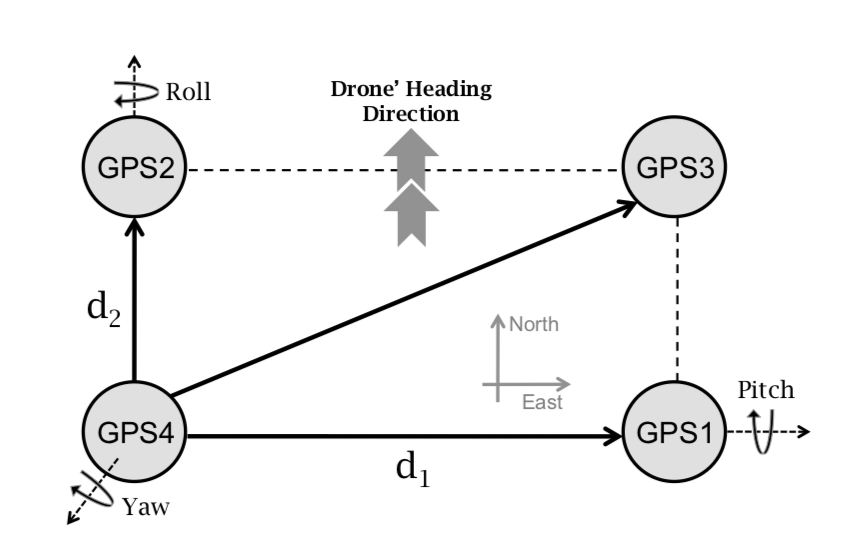
\includegraphics[width=0.6\textwidth]{fig/drone.png}
  \caption{Baseline Matrix}
  \label{drone}
\end{figure}
\subsection{Pseudorange}
Generally, the GPS operates in measuring the the time difference between transmitter
and receive人, also the Pseudorange, which is the estimated distance between both ends
is formed as in equation \ref{p-range}.
\begin{equation}
  Pseudorange = ToF * c
  \label{p-range}
\end{equation}
where $ToF$ is the time difference and $c$ represents the speed of light.\\
However, when a satellite transmits a signal, it includes clock error as the starting time
of transmission is obtained from its atomic clock. The reception time of the
ground receiver is also recorded by less accurate local clock. Because the clock
of a typical GPS receiver is not synchronized to the GPS satellites.
The resulting error can be up to 300 km. GPS signal can get delayed when it enters
the Earth’s atmosphere because of refractions in the Ionosphere and Troposphere.
When signal passes through a multipath channel, more errors would be introduced.
In this study, we model the error in pseudorange at receiver $i$ from the satellite
$s$ as in equation \ref{Pseudorange-model}.
\begin{equation}
  Pseudorange_i^s = \rho_i^s + ct_i - ct^s + A^s + M_i + \epsilon_i^s
  \label{Pseudorange-model}
\end{equation}
Here, $\rho_i^s$ represents the real range, $t_i$ and $t^s$ stand for the clock error at
the receiver and transmitter sides correspondingly. A models the interference by the
atmosphere, $M_i$ stands for the multipath interference and $\epsilon_i^s$ represents
the hardware noise in measuring.\\
The operation error from the system would be as large as 1-4 meters which is far from
satisfaction. Therefore, the Differential GPS technology is introduced leveraging
the difference in signal phase and highly improves the system accuracy.\\
\subsection{Differential GPS}
The differential GPS technology leverages the phase of received GPS signals to improve
the accuracy. One advantage of carrier phase is that its changes over time can
be tracked reliably by utilizing the doppler shift in the signals.\\
The phase model is shown in equation \ref{phase-model} by ignoring the
multipath and hardware noise error. Another advantage of carrier phase is that its changes over time can be tracked reliably by utilizing the doppler shift in the signal.
\begin{equation}
  \lambda\phi_i^s = \rho_i^s + ct_i - ct^s + A^s - N_i^s
  \label{phase-model}
\end{equation}
While $N_i^s$ is Integer Ambiguity,the number of whole cycles on the path from satellite to receiver.[3] The unknown property of $N_i^s$ is called integer ambigity
solve from the phase measurement, and estimating the integer ambiguity is one of the major
concern in the SafetyNet implementation. More discussion on integer ambiguity
would come in later sections.\\
Environmental error sources in Equation 3 are correlated over short time periods
and within small geographical areas (200 km). Thus, two GPS measurements across
time can be subtracted (or differenced) to eliminate some of these factors.
Similarly, simultaneous measurements from multiple GPS receivers can also be
differenced. [4] This study propose 4 kind of differentials.
\subsubsection{Single Differential across Receivers ($SD_{ij}^s(t)$)}

Consider the carrier phase equations for two GPS receivers i and j from the same satellite s (let us ignore multipath and noise).
\begin{equation}
  \begin{split}
    \lambda \bigtriangleup \phi_{ij}^s &= \phi_{i}^s - \phi_{j}^s\\
    &= \bigtriangleup \rho_{ij}^s + c\bigtriangleup t_{ij} - \lambda N_{ij}
  \end{split}
\end{equation}
By differencing the phases at different receivers, correlated error sources of
atmospheric delays and satellite clock biases disappear. \\
For further simplification, $\bigtriangleup \rho_{ij}^s$ is replaced by $\rho_{ij}\cdot \hat{l}_s$,
where $\rho_{ij}$ is the vector between two receivers and $\hat{l}_s$ is the
line-of-sight unit vector from the receiver to the satellite. The transformation
relationship is shown in figure \ref{sdrx}.

\begin{figure}
  \centering
  \captionsetup{justification=centering}
  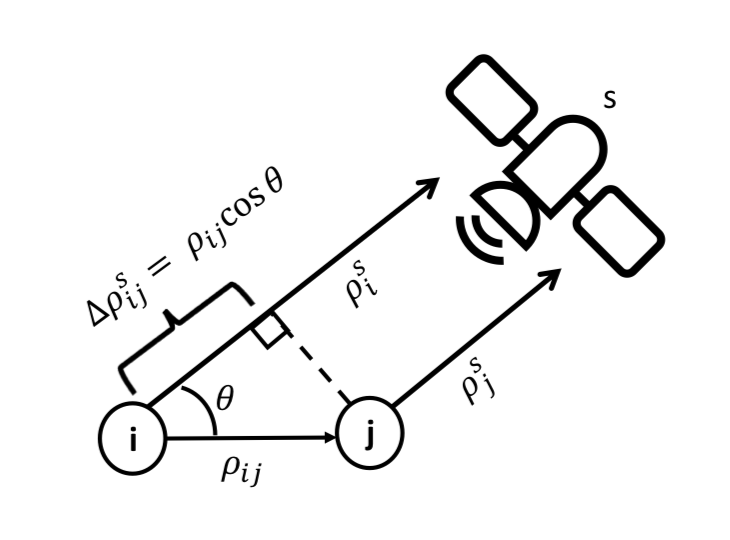
\includegraphics[width=0.6\textwidth]{fig/sdrx.png}
  \caption{$\lambda \bigtriangleup \phi_{ij}^s = \rho_{ij}\cdot \hat{l}_s + c\bigtriangleup t_{ij} - \lambda N_{ij}$}
  \label{sdrx}
\end{figure}

The equation then become:
\begin{equation}
  \lambda \bigtriangleup \phi_{ij}^s = \rho_{ij}\cdot \hat{l}_s + c\bigtriangleup t_{ij} - \lambda N_{ij}
\end{equation}

While by single differential equation, some errors have disappeared,there still exits a function of the clock bias errors, $c\bigtriangleup t_{ij}$ still remains, this call the need for double differentials.

\subsubsection{Double Differential across Receivers and Satellites ($DD_{ij}^{sk}(t)$)}
\begin{equation}
  \begin{split}
    \lambda \bigtriangledown \bigtriangleup \phi_{ij}^{sk}
    &= \lambda \bigtriangleup \phi_{ij}^s - \lambda \bigtriangleup \phi_{ij}^k\\
    &= \rho_{ij}\cdot (\hat{l}_s-\hat{l}_k) - \lambda \bigtriangledown \bigtriangleup N_{ij}^{sk}
  \end{split}
\end{equation}

In this equation, i and j represents two different receivers, and k represents one satellite.
Subtracting the single differential, we get double differential, the the clock biases is removed and the absolute orientation
is achieved, but the residue is polluted by integer ambiguity. \\
In this study, the spatio double differential
forms our measurement model in the filtering process. This paper assume the ambiguities are magically fixed, this provides us a reasonably precise estimate of relative positions between receiver pairs. The technology of Real Time Kinematics (RTK) technology can use the accurately known location of the reference receiver to calculate the location of the other.
\subsubsection{Single Differential across Time ($SD_{i}^{s}(t_{12})$)}
This paper also perform differentials across time for the same receiver. When there is no cycle slips, the equation can be listed as below,
\begin{equation}
  \lambda \bigtriangleup \phi_{i}^s(t_{12}) = \rho_i(t_{12}) \cdot \hat{l}_s + ct_i(t_{12})
\end{equation}

Measurements across 4 satellites can help jointly estimate the relative displacement and clock bias. This
estimated relative displacement is quite accurate since the integer ambiguity $N_i^s$ does not included in it. This paper used
a static receiver placed on the ground to verify the accrancy, and find that the estimation resulted in about $1 cm/s$ of motion.

\subsubsection{Double Differential across Receivers and Time ($DD_{ij}^s(t_1t_2)$)}
By taking the difference between the two single differentials across time,
this paper achieved a measurement of the change in orientation, totally unpolluted by integer ambiguity.
This measurement forms the system transition model in the filtering process. Under the no cycle slips assumption,the interger ambiguity can be elimilated by substracting two equation of single defferential across time.
\begin{equation}
  \begin{split}
  \lambda \bigtriangledown \bigtriangleup \phi_{ij}^{s}(t_{12})
  &= \lambda \bigtriangleup \phi_{i}^s(t_{12}) - \lambda \bigtriangleup \phi_{j}^s(t_{12})\\
  &= (\rho_{ij}(t_1)-\rho_{ij}(t_2)) \cdot \hat{l}_s + c\bigtriangleup t_{ij}(t_{12})
  \end{split}
\end{equation}

\section{System Model}

SafetyNet treat model orientation tracking as a state estimation problem, where the state is defined as 3D orientation and
represent by quaternion.
With both the temporal and spatial differentials, we are able to model the orientation
estimation problem by forming the transition state and absolute measurements.
The system diagram is provided in figure \ref{model}.\\
\begin{figure}
  \centering
  \captionsetup{justification=centering}
  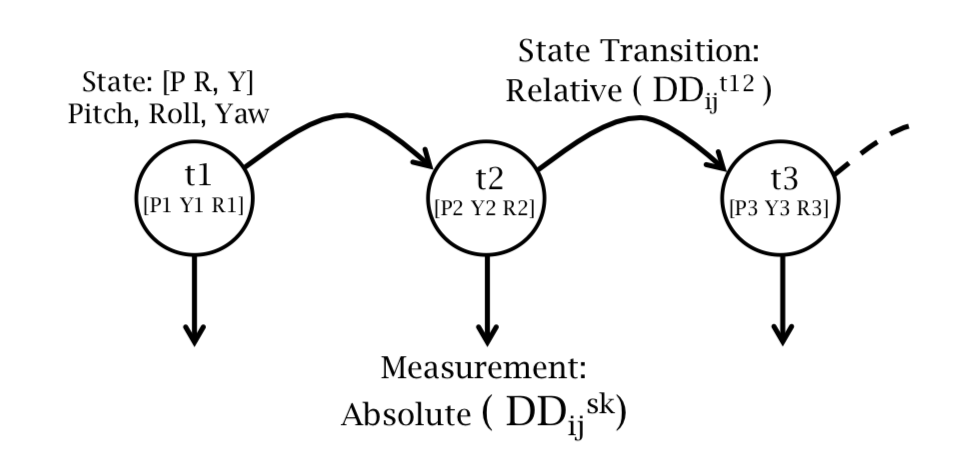
\includegraphics[width=0.6\textwidth]{fig/model.png}
  \caption{System Model}
  \label{model}
\end{figure}
\subsubsection{Transition State}
The temporal differential provides an accurate estimation upon the transition state
as the integer ambiguity is cancelled. By minimizing the relative clock error, we
can solve the equation to track the orientation change $\delta q$ between states.
Here we introduced the 3-dimensional vector representation of orientation $\delta \theta$
whose magnitude is the angle it rotates and direction is the axis it rotates around.
By changing the representation metric, we are able to get rid of the constraint from
quaternion and the estimation becomes a simple Least Square problem:
\begin{equation}
  \lambda \bigtriangledown \bigtriangleup \phi_{ij}^{s}(t_{12})
  = \rho_{ij}(q_0)[A(q_1)\hat{l}_s]_{\times}\delta \theta + c\bigtriangleup t_{ij}(t_{12})
\end{equation}
where $A(q)$ is the rotation matrix corresponding to the quaternion.\\
The solved $\delta \theta$ cannot be directly applied for transition state as the
computation of rotation vector is not immuteable in large scale. We convert it back to
quaternion form and the transition state becomes:
\begin{equation}
  q_{k+1} = \delta q \bigotimes q_{k}
  \label{transition}
\end{equation}
\subsubsection{Absolute State}
The spatial differential is transformed as our absolute measurement at each state.
\begin{equation}
  \lambda \bigtriangledown \bigtriangleup \phi_{ij}^{sk} =
  \rho_{ij}\cdot(\hat{l}_s-\hat{l}_k) + \lambda\bigtriangledown \bigtriangleup N_{ij}
\end{equation}
We can transform the measurement to a function of last state quaternion and a change
in orientation in the vector form.
\begin{equation}
  \lambda \bigtriangledown \bigtriangleup \phi_{ij}^{sk} - \rho_{ij}(q_0)A(q_n)\cdot(\hat{l}_s-\hat{l}_k)
  =  \rho_{ij}(q_0)[A(q_n)\cdot(\hat{l}_s-\hat{l}_k)]_{\times}\delta \theta +
   \lambda\bigtriangledown \bigtriangleup N_{ij}
\end{equation}
The measurement form would be further transformed in Extended Kalman Filter section
for system linearization.
\section{Algorithms}
\subsection{Extended Kalman Filter}
Referring back to equation \ref{transition}, the transition function is intrinsically
a nonlinear operation (the quaternion multiplication),
we make linearized approximations using Extended Kalman Filter (EKF).
Now, linearizing transition model around the estimated rotation vector
associated with quaternion $q_k$ by applying Taylor Expansion, we have:
\begin{equation}
  \delta \theta_{k+1} = F \delta \theta_{k} + \omega_k
\end{equation}
where $\omega_k$ is the system noise.\\
With the linearization process, the absolute state is transformed from absolute
rotation in form of quaternion to change in rotation vector ($\delta \theta$),
as the rotation vector has the property of having muteable operation in small scales and
removes the constraint in magnitude.\\
As with the transition function above, the measurement function can be written
in the following form:\\
\begin{equation}
  y_{k+1}-y_0 = H\delta \theta_{k+1} + v_{k+1}
\end{equation}
where:
\begin{equation}
  y = \lambda \bigtriangledown \bigtriangleup \phi_{ij}^{sk} -
  \lambda\bigtriangledown \bigtriangleup N_{ij}
\end{equation}
\begin{equation}
  y_0 = \rho_{ij}(q_0)A(q_n)\cdot(\hat{l}_s-\hat{l}_k)
\end{equation}
\begin{equation}
  H = \rho_{ij}(q_0)[A(q_n)\cdot(\hat{l}_s-\hat{l}_k)]_{\times}
\end{equation}
and $v_{k+1}$ is the measurement noise.\\

The above EKF has been designed under the convenient assumption that integer ambiguity and cycle slips have been resolved.
However, this resolution is challenging, as evident from the numerous papers written on this topic.[5-7]
The transition model and measurment model can now be combined using an
Extended Kalman Filter for a refined estimate of $\theta^{k+1}$.\\
In the measurement model, the integer ambiguity still exists.
Here we make the assumption that the integer ambiguity is already solved
such that we can ignore it for the filtering process and come back to it afterwards.\\
Once the drone is flying, additional multiples of wavelengths can also accumulate,
called cycle slips. This paper first describe ways to mitigate the initial N and
discuss cycle slips thereafter.\\
Therefore, this paper did not measure integer ambiguity directly, but make it as an index
to identify the estimation they got is correct or not. Their core intuition is
to compute a Cos function on the value of $2\pi N_{ij}^{sk}$,
since $N_{sk}$ should be an integer, $Cos(2\pi N_{sk}^{ij})$ should equal to 1.\\
The process of Kalman filtering is listed as below:
\begin{itemize}
\item Using transition model to get estimation of the next time point: $\delta \theta_{k+1}$.
\item Using measurement model to get the estimation of integer ambiguity.
In an ideal case, the correct q should make the corresponding values of $N_{ij}^{sk}$
equal to 1.
\item Identify the correctness of integer ambiguity using the summation of cosmetrics:
\begin{equation}
  M(q) = \sum_{ij,sk} cos(2\pi N_{sk}^{ij})
\end{equation}
and compare $M(q)$ to the number of possible conbination pairs of receivers $i,j$ and
satellites $s,k$. If $M(q)$ approximates the number we consider it as correct and incorrect
elsewise.
\item If the integer ambiguity is correct, we can continue using kalman filter
to estimate the state.
\item If the integer ambiguity is not correct, the problem is transformed into a
maximization problem. The cosmetric value would always be less than 1 if the estimated
integer ambiguity is not an integer so our intention goes to find the best q to maximize
$M(q)$, i.e.:
\begin{equation}
  q_{coarse} = \argmax_q M(q)
\end{equation}
\item We simply perform a naive grid search in all
3 dimensions of ruler angle (yaw, pitch and roll) with a 5 degree step to find the
optimized solution $q_{coarse}$ to maximize the cosmetric value.
\item After maximization, we update the previous q with $q_{coarse}$, and go back to step 2.
\end{itemize}
The system diagram is shown in figure \ref{kalman}.
\begin{figure}
  \centering
  \captionsetup{justification=centering}
  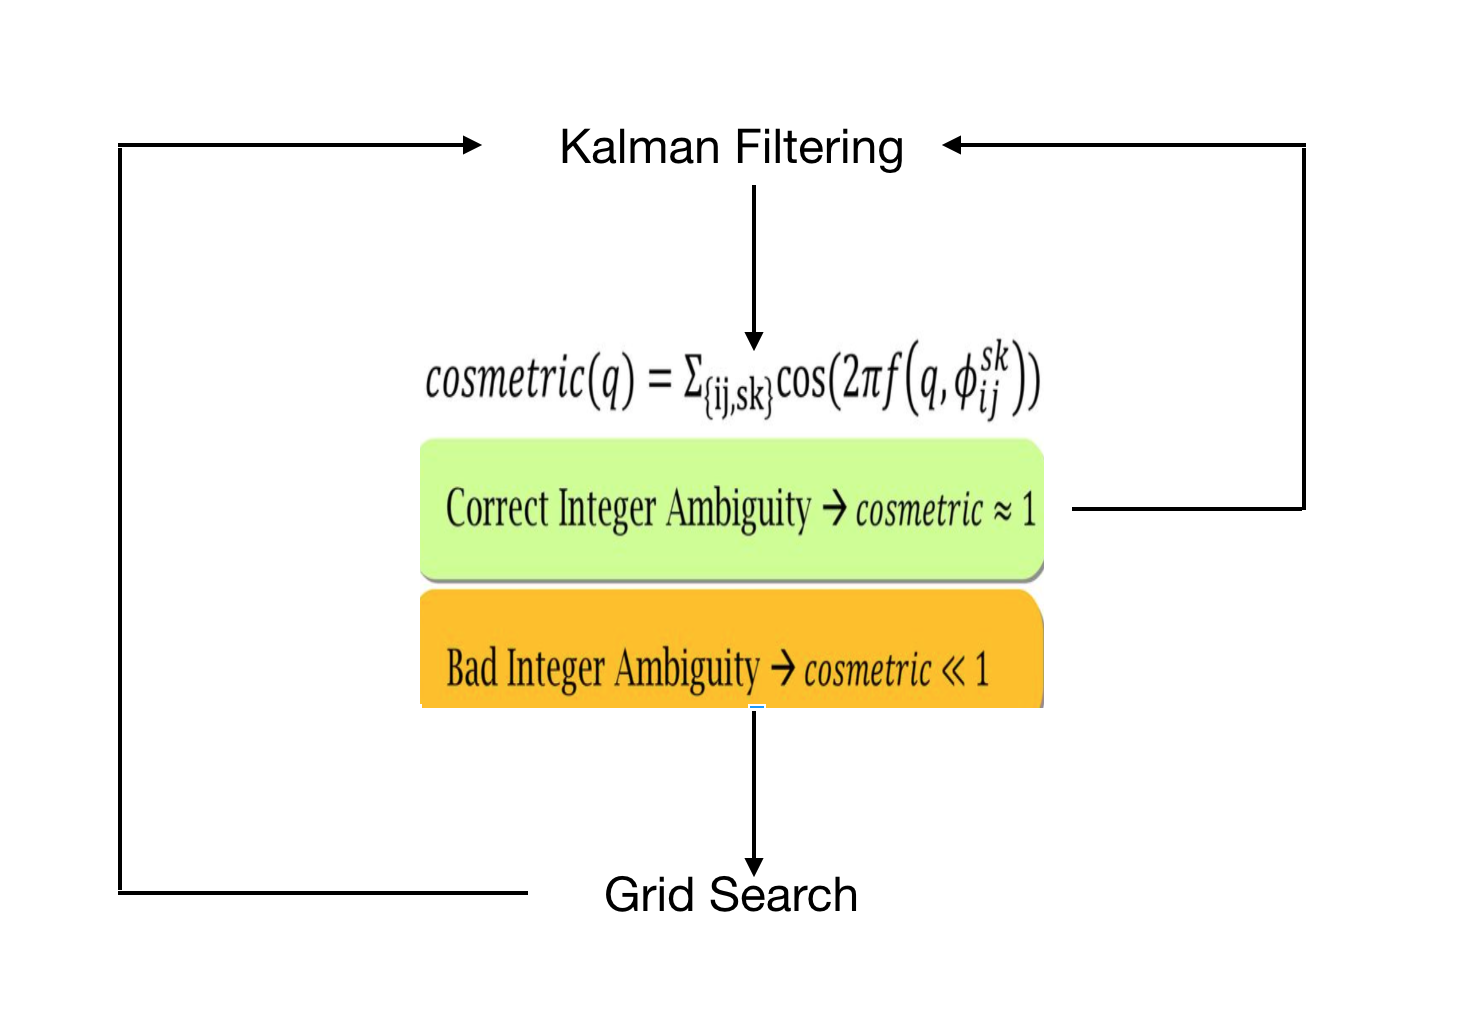
\includegraphics[width=0.6\textwidth]{fig/kalman.png}
  \caption{Kalman Filter}
  \label{kalman}
\end{figure}
\subsection{Advanced Particle Filter}
there exists one phenomenon called cycle slips, A cycle slips causes a jump in
carrier-phase measurements when the receiver phase tracking loops experience a
temporary loss of lock due to signal blockage or some other disturbing factor.
It usually happens with highly aggressive flight drone. The process is listed as follows:
\begin{itemize}
\item Using kalman filtering, we can calculate the cosmetric of each $q_i$
\item if the cosmetric is lower than one, which means the confidence is verified as low,
we switch from kalman filter to particle filter to solve the integer ambiguity problem.
We select K values of orientation q – the values whose corresponding Cos metric ranks
in the top-K. We initialize K particles( from grid search with the top k confidence in
cosmetric form) at each of these orientation states and update them via the transition
model and measurement model.

\item All things goes well, however, there is one problem of the slow convergence
of particle filter. To solve this, this paper develope one advanced particle filter.
In simple particle filter, we propagate to the next stage by transition model,and we
weight them by the measurement model, and assign probability for later use for filtering
and so on. This paper make a simple modification, they move the particle to a state that
maximizes the likelihood,and then perform the resampling step. Thus, the net outcome is
faster convergence for the correct ambiguities, while disappearing particles for incorrect
ambiguities.

\item Upon its convergence, and if the cosmetric close to 1, we switch back to Kalman
filter again.  If the cosmetric is much lower than 1,more particles are added
and resampled – resampling is performed such that the resulting particles are
an equal mix of the (highest weighted) current and new particles, and continuing
the particle filtering process until the cosmetric close to one, and we go back to step one.
\end{itemize}
The system diagram is shown in figure \ref{APF}.
\begin{figure}
  \centering
  \captionsetup{justification=centering}
  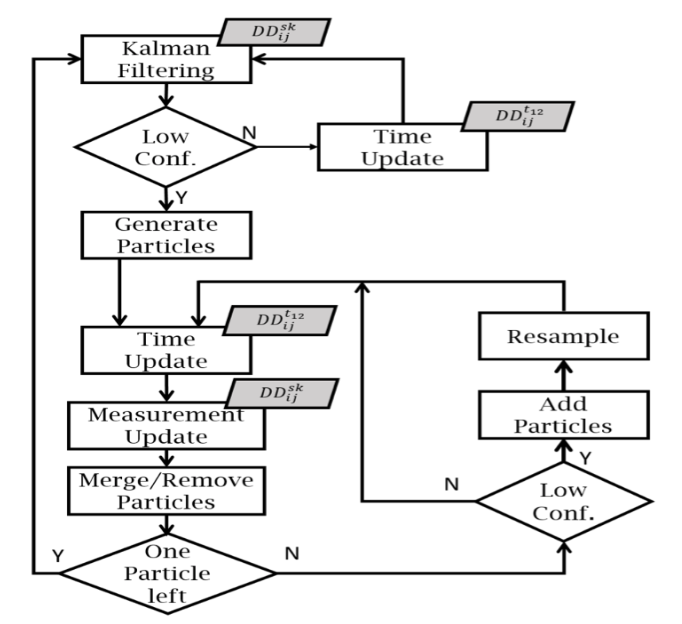
\includegraphics[width=0.6\textwidth]{fig/APF.png}
  \caption{Advanced Particle Filter}
  \label{APF}
\end{figure}
\section{Simulation}
\subsection{Drone Simulation Platform}
The simulation of the base drone is done based on Hector Quatercopter, an open-source
implementation based on Robot Operation System (ROS) and Gazebo.
The platform is shown in figure \ref{hector}.\\
\begin{figure}
  \centering
  \captionsetup{justification=centering}
  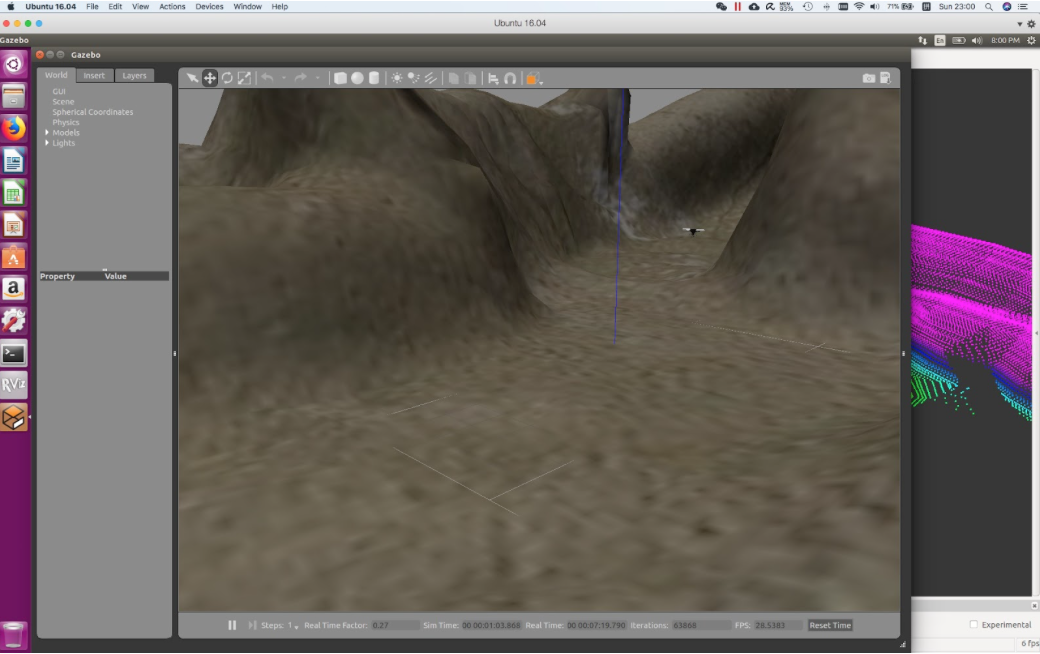
\includegraphics[width=0.6\textwidth]{fig/hector.png}
  \caption{Hector Quatercopter Simulation Platform}
  \label{hector}
\end{figure}
Ground truth data of the location and orientation data is collected to simulate the
multiple GPS receivers attached to the drone.\\
4 GPS receivers are simulated on the 4 arms of the drone, rotated according to
the ground truth orientation and shifted to the real location.\\
Two satellites are fixed on the Medium Earth Orbit and the phases are simulated
from the corresponding distance between the satellite and the receiver.\\
As the drone's movement is relatively ignorable comparing to the distance to the
satellites, the line-of-sight vector is considered as constant.\\
The Kalman and Advanced Particle filters are performed on the simulated data.

\section{Real World Applications}
With the booming applications with unmanned autonomos vechicle, reliable orientation
estimation has been a nontrivial concern. SafetyNet proposes the novel algorithm
to track the orientation with multiple GPS receivers to promise an error of 2 degrees
in environment where magnetic interference and acceleration error accumulates.\\
The reliablity and the accuracy of SafetyNet make it suitable in two major areas of
applications.\\
\paragraph{Reliablity} in the estimation makes it suitable for large quatercopters in aggressive
flying status and in highly interfered magnetic field. Typical applications include
flying in urban area (interference in magnetic field), obstacle avoidance in high
speed flight (error in accelerometers), etc. \\
\paragraph{Accuracy} in orientation estimation powers up the accuracy in
autonomos controll algorithms. For example, accurate tracking of the camera pose make it possible
to achieve better vision-based antonomos flying. 3D reconstruction from the drone's
lens is another application benefits from the accuracy.

\section{Conclusion}

SafeNet use differential techniques, culminating in a novel particle filter framework running over multi-GNSS systems (GPS, GLONASS, and SBAS) to accurately computing the relative locations between each receiver pair, and translating these measurements into the drone’s 3D orientation.Results from 11 sessions of 5-7 minute flights report median orientation accuracies of 2  even under overcast weather conditions. The two filtering algorism used in the paper are Kalman filter and particle filter, we compared the performance of Kalman Filters and Advanced Particle Filter. The performance of Kalman Filters
and Advanced Particle Filters is similar with less aggressive flight, when comes in to highly aggressive flight,
Advanced Particle Filters can better track the drone than Kalman Filter. And after the highly aggressive flight,
Kalman Fliter has large deviation, while Advanced Particle Filters still performs well.
The reason can be listed as below:
\begin{itemize}
\item SafetyNet adopts a hybrid approach to satisfy the linearity and Gaussian assumptions required for Kalman Filter.
\item Missing data in one or more of the receivers derails the state transition function.
\item When the confidence is low, Kalman filter used "grid search" to find the best $q_i$,
this method does not make use of the information from the previous time point and the following time point,
and assume there is only one time point in the cycle slips period.
In comparison, Advanced Particle Filters combines the information from the
previous time point and the following time point, and do not forcefully assign
there is only one time point in cycle slips period.
\end{itemize}

In conclusion, Advanced Particle Filters has better performance than Kalman Filters.




% if have a single appendix:
%\appendix[Proof of the Zonklar Equations]
% or
%\appendix  % for no appendix heading
% do not use \section anymore after \appendix, only \section*
% is possibly needed

% use appendices with more than one appendix
% then use \section to start each appendix
% you must declare a \section before using any
% \subsection or using \label (\appendices by itself
% starts a section numbered zero.)
%


% \appendices
% \section{Proof of the First Zonklar Equation}
% Appendix one text goes here.

% you can choose not to have a title for an appendix
% if you want by leaving the argument blank
% \section{}
% Appendix two text goes here.


% use section* for acknowledgment
% \section*{Acknowledgment}
%
%
% The authors would like to thank...


% Can use something like this to put references on a page
% by themselves when using endfloat and the captionsoff option.
\ifCLASSOPTIONcaptionsoff
  \newpage
\fi



% trigger a \newpage just before the given reference
% number - used to balance the columns on the last page
% adjust value as needed - may need to be readjusted if
% the document is modified later
%\IEEEtriggeratref{8}
% The "triggered" command can be changed if desired:
%\IEEEtriggercmd{\enlargethispage{-5in}}

% references section

% can use a bibliography generated by BibTeX as a .bbl file
% BibTeX documentation can be easily obtained at:
% http://mirror.ctan.org/biblio/bibtex/contrib/doc/
% The IEEEtran BibTeX style support page is at:
% http://www.michaelshell.org/tex/ieeetran/bibtex/
\bibliographystyle{IEEEtran}
% argument is your BibTeX string definitions and bibliography database(s)
%\bibliography{IEEEabrv,../bib/paper}
%
% <OR> manually copy in the resultant .bbl file
% set second argument of \begin to the number of references
% (used to reserve space for the reference number labels box)
\begin{thebibliography}{9}

\bibitem{IMU}
Inertial Measurement Unit: \url{https://en.wikipedia.org/wiki/Inertial\_measurement\_unit}

\bibitem{Mahan}
Mahanth Gowda, Justin Manweiler, Ashutosh Dhekne, Romit Roy Choudhury, and Justin D. Weisz, \emph{Tracking Drone Orientation with Multiple GPS Receivers},\hskip 1em plus
  0.5em minus 0.4em\relax USA, 2016.

\bibitem{Kaplan}
E. Kaplan and C. Hegarty,\emph{Understanding GPS: principles and applications},\hskip 1em plus
  0.5em minus 0.4em\relax ,Artech house, 2005.

\bibitem{Parkinson1}
B. W. Parkinson and P. K. Enge,\emph{"Differential gps,” Global Positioning System: Theory and applications.},\hskip 1em plus
  0.5em minus 0.4em\relax ,vol.~2,~pp.~3–50,~1996.

\bibitem{Parkinson2}
C. E. Cohen and B. W. Parkinson, “Integer ambiguity resolution of the gps carrier for spacecraft attitude determination,” in Guidance and Control 1992, vol. 1, pp. 107–118, 1992.

\bibitem{Conway}
A. Conway, P. Montgomery, S. Rock, R. Cannon, and B. Parkinson, “A new motion-based algorithm for gps attitude integer resolution,” Navigation, vol. 43, no. 2, pp. 179–190, 1996.

\bibitem{Jonge}
P. De Jonge and C. Tiberius, “The lambda method for integer ambiguity estimation: implementation aspects,” Publications of the Delft Computing Centre, LGR-Series, vol. 12, no. 12, pp. 1–47, 1996.

\bibitem{Sutton}
E. Sutton and R. Collins, “Calibration of differential phase map compensation using single axis rotation,” in PROCEEDINGS OF ION GPS, vol. 11, pp. 1831–1842, INSTITUTE OF NAVIGATION, 1998.

\end{thebibliography}

% biography section
%
% If you have an EPS/PDF photo (graphicx package needed) extra braces are
% needed around the contents of the optional argument to biography to prevent
% the LaTeX parser from getting confused when it sees the complicated
% \includegraphics command within an optional argument. (You could create
% your own custom macro containing the \includegraphics command to make things
% simpler here.)
%\begin{IEEEbiography}[{\includegraphics[width=1in,height=1.25in,clip,keepaspectratio]{mshell}}]{Michael Shell}
% or if you just want to reserve a space for a photo:

% \begin{IEEEbiography}{Michael Shell}
% Biography text here.
% \end{IEEEbiography}
%
% % if you will not have a photo at all:
% \begin{IEEEbiographynophoto}{John Doe}
% Biography text here.
% \end{IEEEbiographynophoto}
%
% % insert where needed to balance the two columns on the last page with
% % biographies
% %\newpage
%
% \begin{IEEEbiographynophoto}{Jane Doe}
% Biography text here.
% \end{IEEEbiographynophoto}

% You can push biographies down or up by placing
% a \vfill before or after them. The appropriate
% use of \vfill depends on what kind of text is
% on the last page and whether or not the columns
% are being equalized.

%\vfill

% Can be used to pull up biographies so that the bottom of the last one
% is flush with the other column.
%\enlargethispage{-5in}



% that's all folks
\end{document}
